\subsection{Introducción}
% Describir detalladamente el problema a resolver dando ejemplos del mismo y sus soluciónes.
\par El problema a resolver se trata de una balanza que se encuentra desequilibrada y debemos, por medio de diversas pesas con las que contamos, devolverle el equilibrio.
\par La balanza, en un principio, se encontraba en equilibro. Quitaron una llave (de la cual conocemos su peso) de en uno de los platillos y la balanza se desequilibró. Por suerte, contamos con una serie de pesas con la particularidad de que todos sus pesos son potencias de 3 y no hay repetidas. Por lo tanto queremos determinar qué pesas se deben colocar en cada platillo para reestablecer el equilibrio.
\par Siendo mas específicos,  a partir de una entrada P = `Peso de la llave quitada' de tipo entero debemos encontrar una combinación de potencias de 3 multiplicadas por +1 o -1 nos de como resultado P. Esto se resume en:

\begin{equation}
	\forall P \in \mathds{N},\ P = \sum_{i = 0}^{n} 3^{i} * a_i
\end{equation}
\begin{flushright}
	con $a_i \in \{-1, 0 , +1\}$, según el caso\\
	para algún $n \in \mathds{N}_0$
\end{flushright}

\subsection{Idea General de Resolución}

\par Continuando con la notación utilizada en la introducción, vamos a describir el algoritmo que utilizamos para resolver el problema.
\par El valor \textit{n} (exponente máximo de las potencias de 3) que utilizaremos es $\lceil log_{3}(P) \rceil$ (el por qué de la elección de este valor se explicará en el \textit{Lema 2 del Ej2} en la subsección \ref{ssub: lema_ej2_1}).
\par El algoritmo, en primer lugar, determina cuál es el valor de $a_{n} \in \{-1,0,+1\}$. Esto lo hace quedándose con el que cumpla $| P - a_{n} * 3^{n} | < \frac{3^{n}}{2}$ (para comprender el por qué de este valor ver el \textit{Lema 1 del Ej2} en la subsección \ref{ssub: lema_ej2_2}). Luego, reemplaza a $P$ por $P - a_{n} * 3^{n}$ y a $n$ por $n - 1$ y se llama recursivamente con los valores actualizados de $P$ y $n$. Así, va determinando los valores de cada $a_{i}$ (desde $i=n$ hasta $i=0$).

\subsubsection{Ejemplo ej2:}

\par Veamos un ejemplo del funcionamiento del algoritmo. Tomamos como entrada el número $P = 12$, tenemos $n = \lceil log_{3}(12) \rceil = 3$. El algoritmo compara entre los 3 casos posibles para $a_{k}$ y calcula la diferencia con P:

\begin{itemize}
	\item $a_{3} = -1 \rightarrow  12 - (-1) * 3^{3} =$ \textbf{39}.
	\item $a_{3} = 0 \rightarrow  12 - (0) * 3^{3} =$ \textbf{12}.
	\item $a_{3} = +1 \rightarrow  12 - (+1) * 3^{3} =$ \textbf{-15}.
\end{itemize}
\par Como $\frac{3^{3}}{2} = 14,5$, se determina que $a_{3} = 0$. Se actualiza $P = 12$ y $n = n - 1$ y se realizan nuevamente los mismos pasos. Se comparan los 3 casos:

\begin{itemize}
	\item $a_{2} = -1 \rightarrow  12 - (-1) * 3^{2} =$ \textbf{21}.
	\item $a_{2} = 0 \rightarrow  12 - (0) * 3^{2} =$ \textbf{12}.
	\item $a_{2} = +1 \rightarrow  12 - (+1) * 3^{2} =$ \textbf{4}.
\end{itemize}
\par Ahora tenemos que $\frac{3^{2}}{2} = 4,5$, entonces se determina que $a_{2} = +1$. Se actualiza $P = 12 - (+1) * 3^{2} = 4$ y $n = n - 1$ y se continúa. Se comparan los 3 casos:

\begin{itemize}
	\item $a_{1} = -1 \rightarrow  4 - (-1) * 3^{1} =$ \textbf{7}.
	\item $a_{1} = 0 \rightarrow  4 - (0) * 3^{1} =$ \textbf{4}.
	\item $a_{1} = +1 \rightarrow  4 - (+1) * 3^{1} =$ \textbf{1}
\end{itemize}
\par En este caso tenemos $\frac{3^{1}}{2} = 1,5$, por lo tanto se determina que $a_{1} = +1$. Actualizamos $P = 3 - (+1) * 3^{1} = 0$. Como $P=0$, terminamos de determinar todos los valores $a_{i}$ necesarios. Entonces nos queda que $12 = (+1) * 3^{2} + (+1) * 3^{1}$.

\subsection{Presentación del algoritmo y demostración de correctitud}

\par Antes que nada, vamos a enunciar dos lemas que nos servirán para entender y demostrar el correcto funcionamiento del algoritmo.

\subsubsection{Lema 1 del Ej2:}
\label{ssub: lema_ej2_1}

\par Queremos probar que dado un $P \in \mathds{N}$ y dado un $k \in \mathds{N}_0$, si $|P| \leq \frac{3^{k+1}}{2} \Longrightarrow \exists a_k \in \{-1,+1,0\}$ tal que $|P + a_i * 3^{k}| \leq \frac{3^{k}}{2}$.

\bigskip

\textbf{Demostración:}
\par Dado $P \in \mathds{N}$, $k \in \mathds{N}_0$ tal que $|P| \leq \frac{3^{k+1}}{2}$. Tenemos 3 posibilidades:
\begin{itemize}
	\item Si $|P| \leq \frac{3^{k}}{2} \Longrightarrow$ cumple con $a_{k}=0$.

	\item Si $P > \frac{3^{k}}{2}$: sabíamos que $P \leq \frac{3^{k+1}}{2}$, entonces tenemos que
	\begin{equation}
		\frac{3^{k}}{2} < P \leq \frac{3^{k+1}}{2}
	\end{equation}
	Sumando $-1 * 3^{k}$ tenemos
	\begin{equation}
		\frac{3^{k}}{2} -1 * 3^{k} < P -1 * 3^{k} \leq \frac{3^{k+1}}{2} -1 \cdot 3^{k}
	\end{equation}
	\begin{equation}
		\Longleftrightarrow -\frac{3^{k}}{2} < P -1 * 3^{k} \leq \frac{3^{k}}{2}
	\end{equation}
	Concluimos entonces que
	\begin{equation}
		| P - a_{k} * 3^k | \leq \frac{3^k}{2}
	\end{equation}
	\begin{flushright}
		con $a_{k} = -1$
	\end{flushright}

	\item Si $P < -\frac{3^{k}}{2}$: sabíamos que $P \geq -\frac{3^{k+1}}{2}$, entonces tenemos que
	\begin{equation}
		-\frac{3^{k+1}}{2} \leq P < -\frac{3^{k}}{2}
	\end{equation}
	\par Sumando $+1 * 3^{k}$ tenemos
	\begin{equation}
		-\frac{3^{k+1}}{2} +1 * 3^{k} \leq P < -\frac{3^{k}}{2} +1 * 3^{k}
	\end{equation}
	\begin{equation}
		\Longleftrightarrow -\frac{3^{k}}{2} \leq P < \frac{3^{k}}{2}
	\end{equation}
	\par Concluimos entonces que
	\begin{equation}
		| P - a_{k} * 3^k | \leq \frac{3^k}{2}
	\end{equation}
	\begin{flushright}
		con $a_{k} = +1$
	\end{flushright}
\end{itemize}
\par De esta manera pudimos ver que en las 3 posibilidades se cumple el lema planteado.

\subsubsection{Lema 2 Ej2}
\label{ssub: lema_ej2_2}

\par Queremos probar que $P \leq \frac{3^{n + 1}}{2}$ con $n = log_{3}(P)\ \forall P \in \mathds{N}_{0}$.

\medskip

\textbf{Demostración:}
\par Tenemos $P \in \mathds{N}_{0}$. Queremos ver que cumple:

\begin{equation}
	P \leq \frac{3^{log_{3}(P) + 1}}{2}
\end{equation}
\begin{equation}
	\Longrightarrow P \leq \frac{3^{log_{3}(P)} * 3}{2}
\end{equation}
\begin{equation}
	\Longrightarrow P \leq \frac{P * 3}{2}
\end{equation}
\begin{equation}
	\Longrightarrow 0 \leq \frac{1}{2} * P
\end{equation}
\par Como $P \in \mathds{N}_{0}$, sabemos que se cumple. Por lo tanto tenemos que $P \leq \frac{3^{n + 1}}{2} \forall P \in \mathds{N}_{0}$ con $n = log_{3}(P)$. Notar que como $log_3(p) \leq  \lceil log_3(p) \rceil \Longrightarrow p \leq \frac{3^{log_{3}(P) + 1}}{2} \leq \frac{3^{\lceil log_{3}(P) \rceil + 1}}{2}$


\bigskip

\par Luego de los dos lemas planteados, podremos demostrar la correctitud del algoritmo usado. Para esto, veamos el pseudocódigo del algoritmo:

\medskip

\SetAlgoLined
\SetKwProg{Fn}{Function}{:}{EndFunction}
\begin{algorithm}[H]
	\label{algo: pseudocodigo_ej2}
	\Fn{DameCombinacion(P: int, exponente: int, listaPositivos: lista(int), listaNegativos: lista(int))}{
		\BlankLine
		\If{$exponente < 0$}{
			return
		}
		\BlankLine
		$potenciaActual \gets potencia[exponente]$\\
		\BlankLine
		\uIf{$| P - (+1) * potenciaActual | < \frac{3^{exponente}}{2}$}{
			\BlankLine
			agregar $exponente$ al principio de $listaPositivos$\\
			$P = P - (+1) * potenciaActual$
			\BlankLine
		}
		\uElseIf{$| P - (-1) * potenciaActual | < \frac{3^{exponente}}{2}$}{
			\BlankLine
			agregar $exponente$ al principio de $listaNegativos$\\
			$P = P - (-1) * potenciaActual$
			\BlankLine
		}
		\BlankLine
		$DameCombinacion$($P$, $exponente - 1$, $listaPositivos$, $listaNegativos$)
		\BlankLine
	}
	\caption{Función encargada de calcular el valor asignado al exponente pasado como parámetro, según el número pasado por parámetro.}
\end{algorithm}

\medskip

\par Analicemos el algoritmo siguiendo el pseudocódigo. En la linea 5 se obtiene la potencia de un arreglo que tiene todas las potencias necesarias. Luego se comparan los casos de $a_k$ (lineas 6, 9) según el criterio del \textit{Lema 1 del Ej2} (subsección \ref{ssub: lema_ej2_1}). Si el valor elegido es $+1$, se agrega el exponente a la lista de exponentes positivos y se actualiza el número $P$. En cambio si el valor elegido es $-1$, se agrega el exponente a la lista de exponentes negativos y se actualiza el número $P$. Si no entró en ninguno de los casos anteriores se determina que el valor de $a_{k}$ es 0. Esto lo podemos asegurar porque el lema nos decía que sí o sí uno de los 3 valores cumple la implicación, como ninguno de los otros dos casos cumplía, sabemos que el 0 si cumple. Luego se llama recursivamente con los valores $P$, $listaPositivos$, $listaNegativos$ y $exponente$ decrementado en 1.
\par Si $P$ y $exponente$ cumplen las condiciones necesarias ($| P | \leq \frac{3^{exponente+1}}{2}$), sabemos que al final de la función se realiza una llamada recursiva a sí misma con valores $P$ y $exponente$ que cumple $| P | \leq \frac{3^{exponente+1}}{2}$ (teniendo en cuenta que $exponente$ se disminuyó en 1). Por lo tanto, al ingresar a la función en la llamada recursiva cumple las condiciones necesarias. Este ciclo se da hasta que $exponente$ es menor que 0 y cuando ocurre eso por el lema 2 $exponente = 0 \Longrightarrow P \leq \frac{3^0}{2} = 0,5 \Longrightarrow P = 0$ y por ende luego de la \'ultima llamada recursiva no quedan m\'as exponentes por calcular. En este caso (en la linea 3) se termina la función.
\par Cabe destacar además, que para cada exponente la función solo se llama una vez. Esto nos asegura que los exponentes no se repitan y solo haya un $a_{k}$ asignado a un exponente.

\medskip

\par Volviendo un poco al problema planteado en la introducción, veamos como se utiliza la función planteada para resolverlo. Vamos a llamar a la función con los valores: $P$ = el peso de la llave; $exponente$ = $log_{3}(P)$; $listaPositivos$ y $listaNegativos$ dos listas vacías. Luego de que la función termine su ejecución (y sus respectivas llamadas recursivas), en las listas $listaNegativos$ y $listaPositivos$ estarán los valores de los exponentes necesarios para equilibrar la balanza.


\subsection{Cota de Complejidad}
%3. Deducir una cota de complejidad temporal del algoritmo propuesto (en funci´on de los par´ametros
%que se consideren correctos) y justificar por qu´e el algoritmo desarrollado para la resoluci´on del
%problema cumple la cota dada. Utilizar el modelo uniforme salvo que se explicite lo contrario.

\par Vamos a dar una cota de complejidad del algoritmo y analizaremos el por qué de ese valor. Para esto observaremos el pseudocódigo del Algoritmo \ref{algo: pseudocodigo_ej2}.
\par Veamos la función \textit{DameCombinacion}. En las linea 2-4 hay una comparación y la salida de la función de costo O(1). Luego, en la linea 5 hay una asignación de una exponencial que tiene costo O(1) dado que se accede a una posici\'on de un arreglo. Las guardas de las lineas 6 y 9 tienen costo O(1). En las lineas 7 y 10 se agregan dos enteros al inicio de dos listas. La implementación utilizada para esas listas nos asegura que esa acción tiene costo O(1). Luego en las lineas 8 y 11 se realizan dos asignaciones con costo O(1). Luego en la linea 12 se ejecuta la llamada recursiva. Por lo tanto, para una ejecución de la función (sin contar la llamada recursiva) se obtiene un costo de O(1).
\par Recordemos que la función es llamada con exponente $log_{3}(P)$, y este exponente se disminuye de a 1 antes de hacer una llamada recursiva. Entonces obtenemos una complejidad O($log_{3}(P)$) * O(DameCombinacion) = 0($log_{3}(P)$) * O(1) = 0($log_{3}(P)$).
\par Luego, para imprimir los resultados en el formato pedido, se recorren las listas $listaNegativos$ y $listaPositivos$. Esto nos lleva O(longitud($listaNegativos$) + longitud($listaPositivos$)). Pero sabemos que a lo sumo se recorren $log_{3}(P)$ exponentes y ninguno se repite, por lo que sabemos entonces que $longitud(listaNegativos) + longitud(listaPositivos) \leq log_{3}(P)$. Por lo tanto imprimir los resultados tiene costo O(log(P)).

\medskip

\par En conclusión, la cota de complejidad del algoritmo utilizado para resolver el ejercicio 2 es \textbf{O(log(P))}.

\medskip

\par Para este problema debíamos cumplir una cota de complejidad O($\sqrt{P}$). Dado que nuestra cota de complejidad es O(log(P))
queremos ver que $O(log(P)) \subset O(\sqrt(P))$.\\

Pasemos $P$ a variable real. veamos la relaci\'on de orden entre las respectivas derivadas \\
\begin{equation}
    (log_3(P))' = \frac{1}{P \cdot ln(3)}
\end{equation}
\begin{equation}
    (\sqrt(P))' = \frac{1}{sqrt(P)}\\
\end{equation}
Veamos que la ecuaci\'on 15 es mayor que la ecuaci\'on 14:
\begin{equation}
        \frac{1}{P \cdot ln(3)} \leq \frac{1}{sqrt(x)}\\
\end{equation}
\begin{equation}
        \Longrightarrow P \cdot ln(3) \geq sqrt(P)\\
\end{equation}

\begin{equation}
        \Longrightarrow \sqrt(P) \cdot ln(3) \geq 1\\
\end{equation}
Es f\'acil ver que la ecuaci\'on 18 se cumple $\forall P > 0$.
Como la derivada de $\sqrt(P)$ es mayor que la de $log_3(P)$ entonces 
\begin{equation}
        lim_{n \to \infty}\frac{log_3(P)}{\sqrt(P)} = 0
\end{equation}
Entonces $O(log(P)) \subset O(\sqrt(P))$ $\square$ \\
Por la demostraci\'on de arriba se cumpli\'o con la cota pedida.

\subsection{Experimentaci\'on}
Como se puede ver en la figura nuestra hipotesis de que la complejidad de nuestro algoritmo es $O(log(P))$ se verifica.

\begin{figure}
	\centering
	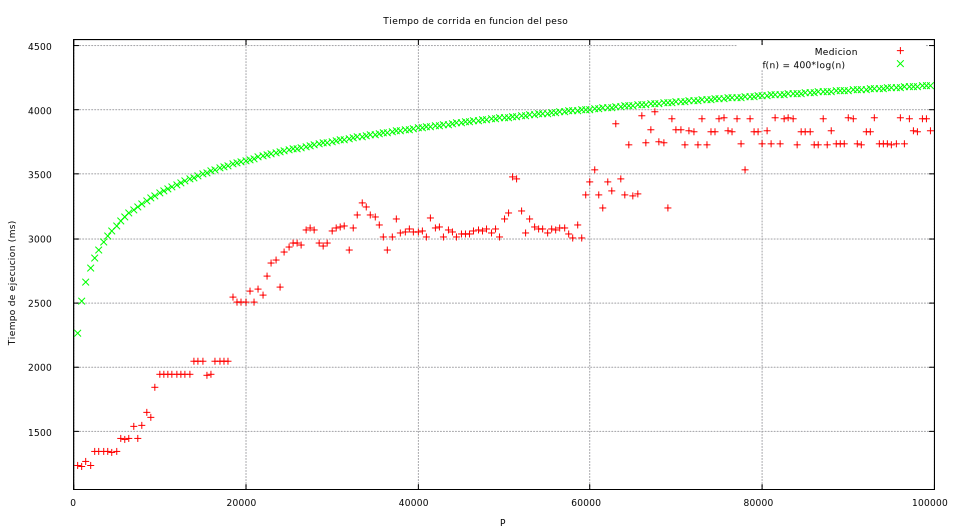
\includegraphics[width=1\textwidth]{images/graficoposta.png}
	\caption{Gr\'afico del tiempo de ejecuci\'on con respecto a $log(p)$}
	\label{}
\end{figure}

